\documentclass[final]{ijpp}

  \usepackage[final,dvips]{graphicx}
  \usepackage{latexsym}
  \usepackage{mathptmx}
  \usepackage{url} 
  \usepackage{setspace}
  \usepackage{epsfig}
  
  \begin{document}

  \title{Language and Compiler Design for Streaming Applications}   
  \titlerunning{Language and Compiler Design for Streaming Applications}

  \author{Saman Amarasinghe, Michael I. Gordon, Michal Karczmarek,
	    Jasper Lin, David Maze, Rodric M. Rabbah, and William Thies}

  \institute{Computer Science and Artificial Intelligence Laboratory,
	       Massachusetts Institute of Technology,
		 Cambridge, MA 02139.
		 Email: \{saman, mgordon, karczma, jasperln, dmaze, rabbah, thies\}@csail.mit.edu}
  \authorrunning{Amarasinghe et al.}
 
  \urldef\streamiturl\url{http://www.cag.csail.mit.edu/streamit/}

  \maketitle
  \bibliographystyle{ijpp}

  \begin{abstract}
  High-performance  streaming  applications  are  a new  and  distinct
  domain  of programs  that is  increasingly important.   The StreamIt
  language  provides  novel   high-level  representations  to  improve
  programmer productivity and  program robustness within the streaming
  domain.  At the same time, the StreamIt compiler aims to improve the
  performance of  streaming applications via  stream-specific analysis
  and  optimizations.   In  this  paper, we  motivate,  describes  and
  justify the  StreamIt language which  include a structured  model of
  streams,  a messaging  system  for control,  and  a natural  textual
  syntax.
  \end{abstract}

  \begin{keywords}
  Stream computing; StreamIt; parallelizing compiler;
  tiled-processor architectures; productivity.
  \end{keywords}

\clearpage

\doublespacing


\section{Introduction}
\label{sec:intro}

Applications that  are structured around  some notion of  a ``stream''
are  prevalent to common computing practices, and there is
evidence   that  streaming  media   applications  already   consume  a
substantial fraction  of the  computation cycles on  consumer machines
\cite{rixner98bandwidthefficient}. Furthermore, stream processing---of
voice and video  data---is central to a plethora  of embedded systems,
including  hand-held  computers, cell  phones,  and  DSPs. The  stream
abstraction is  also fundamental  to high-performance systems  such as
intelligent  software  routers, cell  phone  base  stations, and  HDTV
editing consoles.

Despite the  prevalence of  these applications, there  is surprisingly
little language and compiler support for practical, large-scale stream
programming.   Of course,  the notion  of  a stream  as a  programming
abstraction was  established decades ago \cite{SICP}, and  a number of
special-purpose stream languages  exist today (see \cite{survey97} for
a review).   Many of these  languages and representations  are elegant
and theoretically sound,  but they are not flexible  enough to support
straightforward development  of modern stream  applications, and their
implementations are too inefficient to use in practice.  Consequently,
most programmers resort to general-purpose  languages such as C or C++
to  implement stream  programs.   Yet there  are  several reasons  why
general-purpose languages are  inadequate for stream programming. Most
notably, they do not provide  a natural or intuitive representation of
streams,  thereby  reducing  readability, robustness,  and  programmer
productivity.   Moreover,  because   the  widespread  parallelism  and
regular communication  patterns of data  streams are left  implicit in
general-purpose  languages,  compilers  are not  stream-conscious  and
cannot   perform   stream-specific   optimizations.   As   a   result,
performance-critical codes are often expressed in a low-level assembly
language  and must  be  re-implemented for  each target  architecture.
This practice is labor-intensive, error-prone, and very costly.

General-purpose  languages are  also  poorly suited  for the  emerging
class of  tile-based architectures \cite{smartmemories,rawshort,trips}
that  are  well-geared for  stream  processing.   Perhaps the  primary
appeal  of C is  that it  provides a  ``common machine  language'' for
von-Neumann   architectures.    That  is,   it   abstracts  away   the
idiosyncratic  differences between  machines,  but encapsulates  their
common  properties: a single  program counter,  arithmetic operations,
and a monolithic memory.  However, the von-Neumann model does not hold
in  the   context  of  tiled  architectures  as   there  are  multiple
instruction streams and distributed  memory banks. Consequently, C can
not serve  as a common machine  language, and in fact  it provides the
wrong    abstraction     for    the    underlying     hardware,    and
architecture-specific directives are often needed to obtain reasonable
performance.   Thus   the  responsibilities  of   the  programmer  are
increased, and the portability of applications is hampered.

In  this paper,  we describe  and  justify StreamIt  as a  high-level,
architecture independent  programming language for  stream programming
(Section~\ref{sec:overview}).   The StreamIt  language is  designed to
provide  high-level   stream  abstractions  that   improve  programmer
productivity  and  program  robustness  within the  streaming  domain.
Furthermore, it is intended to  serve as a common machine language for
tile-based  processors, and parallel  computing substrates  in general
(e.g., grids  and clusters  of workstations).  At  the same  time, the
StreamIt compiler aims  to perform novel stream-specific optimizations
to    achieve    the    performance    of   an    expert    programmer
(Section~\ref{sec:compiler}).

In  the following  section, we  begin with  a characterization  of the
streaming    domain   and   motivate    the   design    of   StreamIt.
Section~\ref{sec:related}     discusses      related     work,     and
Section~\ref{sec:conc} summarizes and concludes the paper.


\section{Streaming Application Domain}
\label{sec:domain}

The applications  that make use  of a stream abstraction  are diverse,
with targets  ranging from embedded devices, to  consumer desktops, to
high-performance servers.  Examples include  systems such as the Click
modular router \cite{click} and the Spectrumware software radio
\cite{spectrumware,softwareradio};   specifications    such   as   the
Bluetooth communications protocol \cite{bluetooth}, the GSM Vocoder
\cite{gsm}, and the AMPS cellular base station\cite{amps}; and almost
any application developed with Microsoft's DirectShow library
\cite{directshow}, Real Network's RealSDK \cite{realsdk} or Lincoln
Lab's Polymorphous Computing Architecture \cite{pca}.


We  have identified a  number of  properties that  are common  to such
applications---enough  so as to  characterize them  as belonging  to a
distinct class of  programs which we will refer  to as \emph{streaming
applications}.   We  believe that  the  salient  characteristics of  a
streaming application are as follows:

\begin{enumerate}
\item \emph{Large streams of data.}  Perhaps the most fundamental
  aspect of a streaming application is that it operates on a large (or
  virtually infinite) sequence of data items, hereafter referred to as
  a \emph{data stream}.  Data streams generally enter the program from
  some external source, and each  data item is processed for a limited
  time  before being  discarded.  This  is in  contrast  to scientific
  codes which  manipulate a  fixed input set  with a large  degree of
  data reuse.

\item \emph{Independent stream filters.}  Conceptually, a streaming
  computation  represents a  sequence of  transformations on  the data
  streams in  the program.  We  will refer to  the basic unit  of this
  transformation  as  a  \emph{filter}:  an operation  that---on  each
  execution  step---reads one  or  more items  from  an input  stream,
  performs some computation, and writes one or more items to an output
  stream.   Filters  are  generally  independent  and  self-contained,
  without references  to global variables or other  filters.  A stream
  program is the composition of filters into a \emph{stream graph}, in
  which the  outputs of  some filters are  connected to the  inputs of
  others.
  
\item \emph{A stable computation pattern.}  The structure of the
  stream graph is generally constant during the steady-state operation
  of  a  stream  program.  That  is,  a  certain  set of  filters  are
  repeatedly  applied in a  regular, predictable  order to  produce an
  output stream that is a given function of the input stream.
  
\item \emph{Occasional modification of stream structure.}  Even though
  each arrangement of  filters is executed for a  long time, there are
  occasional dynamic modifications to the stream graph.  For instance,
  a software radio re-initializes a portion of the stream graph when a
  user switches  from AM  to FM.  Sometimes,  these re-initializations
  are synchronized  with some  data in the  stream, as when  a network
  protocol changes  from Bluetooth to 802.11  at a certain  point of a
  transmission.    There  is   typically  an   enumerable   number  of
  configurations that the  stream graph can adopt in  any one program,
  such that all  of the possible arrangements of  filters are known at
  compile time.
  
\item \emph{Occasional out-of-stream communication.}  In addition to
  the  high volume data streams  passing from  one filter  to another,
  filters also communicate small  amounts of control information on an
  infrequent  and  irregular  basis.   Examples include  changing  the
  volume on  a cell phone, printing  an error message to  a screen, or
  changing a coefficient in an upstream FIR (Finite Impulse Response) filter.
  
\item \emph{High performance expectations.}  Often there are real-time
  constraints that must be  satisfied by streaming applications. Thus,
  efficiency (in  terms of both  latency and throughput) is  a primary
  concern.  Additionally, many  embedded applications are intended for
  mobile  environments where  power consumption,  memory requirements,
  and code size are also important.
\end{enumerate}


\section{Language Overview}
\label{sec:overview}

StreamIt  includes  stream-specific  abstractions and  representations
that are designed to improve programmer productivity in the domain of
streaming   applications.   StreamIt   programs  are   represented  as
hierarchical  stream  graphs   consisting  of  \emph{filters}  as  the
fundamental processing  blocks. This section
presents the StreamIt 2.0 syntax for describing filters and the stream
graph.

%%%%%%%%%%%%%%%%%%%%%%%%%%%%%%%%%%%%%%%%%%%%%%%%%%%%%%%%%%%%%%%%%%%%%%
\subsection{Filters}

The basic unit of computation  in StreamIt is the \texttt{filter}.  An
example   of  a   \texttt{filter}   from  our   software  radio   (see
Fig.~\ref{fig:radiodiagram})  is  the  \texttt{FIRFilter}, shown  in
Fig.~\ref{fig:firstreamit}.  Each  filter has an  input channel from
which it  reads data, and an  output channel to which  it writes data.
The filter also contains a \texttt{work} function, which describes the
filter's most fine grained execution step in the steady state.  Within
the \texttt{work} function, a  filter can communicate with neighboring
blocks  over  implicit  channels  that support  three  operations:  1)
\texttt{pop()} removes an item from the end of the channel and returns
its value,  2) \texttt{peek($i$)}  returns the value  of the  item $i$
spaces  from  the end  of  the channel  without  removing  it, and  3)
\texttt{push($x$)}  writes  $x$ to  the  front  of  the channel.   The
argument $x$ is  passed by value; if it is an  object, a separate copy
is enqueued  on the  channel. Currently, the  number of  items peeked,
popped, and pushed by each filter must be constant from one invocation
of the \texttt{work}  function to the next.  In  fact, as described in
the sequel,  the input and  output rates are  declared as part  of the
\texttt{work} function declaration; a  violation of the declared rates
may  result in  a runtime  error and  the subsequent  behavior  of the
program is  undefined. We plan  to support variables input  and output
rates in a future version of StreamIt.

Each filter also contains an  \texttt{init} function that is called at
the time  of initialization.  This  function allows the  programmer to
establish the initial state of the filter.  For example, the FIRFilter
calculates some  \texttt{weights} that will serve  as coefficients for
filtering.   The \texttt{init}  function may  not push,  pop,  or peek
items; however, a filter  may also declare a \texttt{prework} function
to  be called in  place of  the normal  \texttt{work} function  on the
first  iteration.   A   filter  is  instantiated  using  \texttt{add},
\texttt{body},  or  \texttt{loop}  statements, and  the  \texttt{init}
function is called implicitly with the same arguments that were passed
in the instantiating statements.

Each filter has  a fixed input type, output type,  and I/O rates.  The
input  and  output   types  are  specified  as  part   of  the  filter
declaration;  the sample  \texttt{FIRFilter} has  an input  and output
type         of         \texttt{float},         represented         as
\texttt{float}~$\rightarrow$~\texttt{float}.   The I/O rates  are declared
as part of the work function.   Any expression that can be resolved to
a constant at compile time is a  valid I/O rate.  The peek rate may be
omitted if it is the same as the pop rate.

\subsubsection{Rationale}  
StreamIt's  representation   of  a  filter  is   an  improvement  over
general-purpose languages.  In a  procedural language, the analog of a
filter  is a  block  of statements  in  a complicated  loop nest  (see
Fig.~\ref{fig:firprocedural}).  This representation is unnatural for
expressing the feedback and  parallelism that is inherent in streaming
systems.   Also, there  is no  clear abstraction  barrier  between one
filter and another, and  high-volume stream processing is muddled with
global variables and control flow.   The loop nest must be re-arranged
if  the input  or output  ratios of  a filter  change,  and scheduling
optimizations  further  inhibit  the  readability  of  the  code.   In
contrast,  StreamIt places  the filter  in its  own  independent unit,
making explicit  the parallelism and  inter-filter communication while
hiding  the grungy  details of  scheduling and  optimization  from the
programmer.

Alternatively, one could use  an object-oriented language to implement
a  stream abstraction  (see Fig.~\ref{fig:firobject}).   This avoids
some of the  problems associated with a procedural  loop nest, but the
programming model  is again complicated by  efficiency concerns.  That
is, a  runtime library  usually executes filters  according to  a pull
model, where  a filter operates on  a block of data  that it retrieves
from the  input channel.   The block size  is often optimized  for the
cache  size  of  a  given architecture,  thus  hampering  portability.
Moreover, operating  on large-grained blocks  obscures the fundamental
fine-grained algorithm  that is visible  in a StreamIt  filter.  Thus,
the absence  of a runtime model  in favor of  automated scheduling and
optimization again distinguishes StreamIt.

\subsection{Connecting Filters}
\label{sec:connecting}

StreamIt  provides  three  constructs  for composing  filters  into  a
communicating network. They are \texttt{pipeline}, \texttt{splitjoin},
and  \texttt{feedbackloop}  (see Fig.~\ref{fig:structuresp}).   Each
structure  specifies a pre-defined  way of  connecting filters  into a
single-input,  single-output  block,   henceforth  refereed  to  as  a
``stream'';   a  stream   is  any   instance  of   a  \texttt{filter},
\texttt{pipeline},  \texttt{splitjoin},  or \texttt{feedbackloop}.   A
pipeline is  for building a sequence  of streams, a  split-join is for
running streams  in parallel,  and a feedback  loop is  or introducing
cycles in the stream graph.   Every StreamIt program is a hierarchical
composition of these stream structures.

The \texttt{pipeline} construct is for building a sequence of streams.
The body of  a pipeline is a sequence of  statements that are executed
upon its  instantiation.  Component streams are added  to the pipeline
via   successive  calls   to  \texttt{add}.    For  example,   in  the
\texttt{AudioEcho} in Fig.~\ref{fig:echo}, there are four streams in
the  pipeline:  an  \texttt{AudioSource}, an  \texttt{EchoEffect},  an
\texttt{Adder}, and  a \texttt{Speaker}.  This  sequence of statements
automatically connects the four streams in the order specified.  There
is  no \texttt{work}  function in  a pipeline:  the  component streams
fully specify the behavior; the  channel types and data rates are also
implicit from the connections.

The  \texttt{splitjoin}  construct  is  used  to  specify  independent
parallel streams that diverge  from a common \emph{splitter} and merge
into a  common \emph{joiner}.  As in  a pipeline, the  components of a
split-join are  specified with successive calls  to \texttt{add}.  For
example,  the \texttt{EchoEffect}  in  Fig.~\ref{fig:echo} adds  two
streams that run in parallel, the first is a \texttt{Delay} filter and
the other is an identity filter.

The splitter specifies how items  from the input of the split-join are
distributed to  the parallel components. Currently we  allow two types
of  compiler-defined  splitters:  \texttt{duplicate} which  replicates
each  data  item  and  sends  a  copy to  each  parallel  stream,  and
\texttt{roundrobin($i_1$,  $i_2$,  $\dots$,  $i_k)$} which  sends  the
first $i_1$  data items to the  stream that was added  first, the next
$i_2$ data items  to the stream that was added second,  and so on.  As
shorthand,      \texttt{roundrobin($i$)}     is      equivalent     to
\texttt{roundrobin($i$,    $i$,   $i$,   $\dots$)}.     An   unadorned
\texttt{roundrobin} is  equivalent to \texttt{roundrobin(1)}.  Lastly,
if none of the parallel components require any input, and there are no
input items  to split, then \texttt{roundrobin(0)} may  be used.  Note
that \texttt{roundrobin} can function  as an exclusive selector if one
or more of the weights are zero.

Similarly,  the joiner  is used  to indicate  how the  outputs  of the
parallel  streams  are  interleaved  on  the  output  channel  of  the
split-join.  The  only supported joiner  is \texttt{roundrobin}, which
is analogous to a round-robin splitter.

The   splitter  and  joiner   types  are   specified  with   calls  to
\texttt{split}      and     \texttt{join},      respectively.      The
\texttt{EchoEffect}  uses  a  duplicate  splitter so  that  each  item
appears directly---via the identity  filter---and as an echo---via the
\texttt{Delay}   filter.  The   round-robin  joiner   interleaves  the
immediate signals  with the  delayed ones.  In  \texttt{AudioEcho}, an
\texttt{Adder} is used to combine each pair of interleaved signals.

The \texttt{feedbackloop} construct provides a way to create cycles in
the    stream    graph.      The    \texttt{Fibonacci}    stream    in
Fig.~\ref{fig:feed}  illustrates the  use of  this  construct.  Each
feedback loop  contains: 1) a body  stream, which is  the block around
which a backward ``feedback path'' is being created, 2) a loop stream,
which  can perform  some computation  along  the feedback  path, 3)  a
splitter,  which distributes data  between the  feedback path  and the
output  channel at  the bottom  of the  loop, and  4) a  joiner, which
merges items  between the feedback path  and the input  channel at the
top  of  the  loop.   These  components are  specified  via  calls  to
\texttt{body},   \texttt{loop},  \texttt{split},   and  \texttt{join},
respectively.

The   splitters   and   joiners   can   be  any   of   those   for   a
\texttt{splitjoin}, with the exception of \texttt{roundrobin(0)}.  The
call to  \texttt{loop} may be  omitted if no computation  is performed
along the feedback path.

The  feedback loop  has special  semantics  when the  stream is  first
executed.   The loop's  joiner  needs inputs  from  its feedback  path
before  it can fire.   These inputs  are provided  by \texttt{enqueue}
statements within the body of the loop.

Evident in the \texttt{Fibonnacci} example of Fig.~\ref{fig:feed} is
another  feature   of  the  StreamIt   syntax:  \emph{inlining}.   The
definition  of  any  stream  can  be  inlined  at  the  point  of  its
instantiation, thereby preventing the  definition of many small stream
structures that are used only  once, and, moreover, providing a syntax
that  reveals  the hierarchical  structure  of  the  streams from  the
indentation level of the code.

\subsubsection{Rationale}
StreamIt  differs   from  other  languages   in  that  it   imposes  a
well-defined structure on the streams; all stream graphs are built out
of a hierarchical composition  of pipelines, split-joins, and feedback
loops.   This is  in  contrast to  other  environments that  generally
regard a  stream as a flat  and arbitrary network of  filters that are
connected  by  channels.   Arbitrary  graphs  are very  hard  for  the
compiler  to  analyze,  and  equally  difficult for  a  programmer  to
describe.  Most  programmers either resort to  straight-line code that
links one filter  to another (thereby obscuring the  stream graph), or
they use  an ad-hoc graphical  programming environment that  admits no
good textual representation.

In contrast, StreamIt affords a clean textual representation of stream
graphs,  and the  comparison  of StreamIt's  structure with  arbitrary
stream  graphs may  be likened  to the  difference  between structured
control  flow  and  GOTO   statements:  although  the  structure  may
occasionally restrict the expressiveness  of the programmer, the gains
in  robustness,  readability,   and  compiler  analysis  are  immense.
Furthermore, the  graphical programming environment  we have developed
for StreamIt has the advantage  that every stream graph corresponds to
a precise textual  counterpart that is easily edited  by a programmer.
Further,  the hierarchical  structure of  the stream  graph simplifies
visualization,  and  hence  the  graphical development  environment  is
better suited for large scale application development.

\subsection{Messages}

StreamIt provides  a dynamic  messaging system for  passing irregular,
low-volume control information  between filters and streams.  Messages
are sent  from within the  body of a filter's  \texttt{work} function,
perhaps to change a parameter  in another filter.  For example, in our
software  radio  example,  the  \texttt{CheckFreqHop}  stage  sends  a
message upstream to change the frequency of the receiver if it detects
that the transmitter  is about to change frequencies.   The sender can
continue  to execute while  the message  is en  route, and  the target
method will  be invoked in  the receiver with the  specified arguments
when  the message  arrives.  Since  message delivery  is asynchronous,
there  can  be no  return  value; only  void  methods  can be  message
targets.

The central aspect  of the messaging system is  a sophisticated timing
mechanism that  allows filters to  specify when a message  is received
relative  to  the flow  of  information  between  the sender  and  the
receiver.  Recall that each filter executes independently, without any
notion of global  time.  Thus, the only meaningful  notion of time for
any two filters is in terms  of the data items that are passed through
the streams from one to the other.

In StreamIt,  one can  specify a range  of latencies for  each message
delivery.   This  latency  is  measured  in terms  of  an  information
``wavefront''  from  one  filter  to  another.  For  example,  in  the
\texttt{CheckFreqHop}  example  of Fig.~\ref{fig:radiodiagram},  the
sender indicates  an interval of  latencies e.g. between $4$  and $6$.
Due to space limitations, we  cannot define this notion precisely (see
\cite{streamittech620,streamittech622} for  the formal semantics), but
the general idea  is simple: the receiver is invoked  when it sees the
information wavefront  that the  sender sees in  $4$ to  $6$ execution
steps.

StreamIt  also supports  modular broadcast  messaging.  When  a sender
wants to  send a message that  will invoke method $M$  of the receiver
$R$ upon arrival, it does not  call $M$ on the object $R$.  Rather, it
calls $M$  on a \emph{portal} of  which $R$ is a  member.  Portals are
typed  containers  that  forward  all  messages they  receive  to  the
elements of  the container.  Portals could  be useful in  cases when a
component of a filter library  needs to announce a message (e.g., that
it is  shutting down) but  does not know  the list of  recipients; the
user of  the library can  pass to the  filter a portal  containing all
interested receivers.   As for message delivery  constraints, the user
specifies a single  time interval for each message,  and that interval
is interpreted  separately (as described  above) for each  receiver in
the portal.

\subsubsection{Rationale}
Stream  programs present  a challenge  in that  filters  need regular,
high-volume  data transfer  as well  as irregular,  low-volume control
communication.  Moreover, there is  the problem of reasoning about the
relative ``time'' between filters when they are running asynchronously
and in parallel.

A different approach to messaging  is to embed control messages in the
data  stream instead  of providing  a separate  mechanism  for dynamic
message passing.  This does have the effect of associating the message
time with a  data item, but it is  complicated, error-prone, and leads
to unreadable code.  Further, it  could hurt performance in the steady
state  (if each filter  has to  check whether  or not  a data  item is
actual  data or  control, instead)  and may  also  complicate compiler
analysis.  Finally, one can't  send messages upstream without creating
a separate data channel for them to travel in.

Another  solution is to  treat messages  as synchronous  method calls.
However, this delays the progress of the stream when the message is en
route,  thereby   degrading  the   performance  of  the   program  and
restricting the compiler's freedom to reorder filter executions.

We feel  that the StreamIt  messaging model is  an advance in  that it
separates   the   notions   of   low-volume   and   high-volume   data
transfer---both for the programmer and the compiler---without losing a
well-defined semantics where messages are \emph{timed} relative to the
high-volume data  flow.  Further, by  separating message communication
into its  own category, fewer connections are  needed for steady-state
data transfer  and the  resulting stream graphs  are more  amenable to
structured stream programming.


\section{StreamIt Compiler}
\label{sec:compiler}

We  have  implemented  a  fully-functional  StreamIt  compiler  as  an
extension to  the Kopi Java  Compiler, a component of  the open-source
Kopi   Project\cite{kopi}.   The   compiler  performs   a   number  of
stream-specific optimizations, and targets a conventional uniprocessor
machine,  a  networked  cluster   of  workstations,  or  the  MIT  Raw
architecture.  Raw consists  of a 2D mesh of  16 independent processor
tiles with fast  statically scheduled interconnect\cite{rawshort}.  We
have also developed a library that allows StreamIt code to be executed
as pure Java, thereby providing a rapid verification mechanism.

The  compilation process  for streaming  programs contains  many novel
aspects because the basic unit  of computation is a stream rather than
a procedure.  In  order to compile stream modules  separately, we have
developed a runtime interface---analogous  to that of a procedure call
for  traditional codes---that specifies  how one  can interact  with a
black  box of  streaming computation.   The stream  interface contains
separate phases for initialization  and steady-state execution; in the
execution phase,  the interface includes  a contract for  input items,
output items, and possible message production and consumption.

Compiling for Raw involves  constructing an expanded stream graph from
the input program, and then  partitioning this into 16 sections to fit
on to  the tiles of the chip\cite{gordon02}.   The principal technique
for doing  this involves \emph{fusing} adjacent filters  in the stream
graph to form a single filter.  \emph{Vertical fusion} performs fusion
on successive  filters in  a pipeline, while  \emph{horizontal fusion}
joins the parallel streams in a split-join.

The  StreamIt   compiler  also  contains  a   set  of  domain-specific
optimizations for linear  filters where each output is  a weighted sum
of  the  inputs (e.g.,  FIR,  FFT,  DCT).  The compiler  automatically
detects   linear   filters    and   performs   large-scale   algebraic
simplification   of  adjacent   components,  as   well   as  automated
translation into the frequency  domain when the transformation results
in faster code.  These techniques  yield average speedups of 450\% for
benchmarks  with   large  linear  components;   see~\cite{lamb03}  for
details.

We    have     implemented    a    number     of    stream    programs
(Table~\ref{tab:benchmarks}) to test  the performance of our compiler.
Our benchmarks include several  small kernels which would typically be
used as parts of larger applications, along with some larger systems.

Results of the compiler are given in Table~\ref{tab:performance}.  For
each  application,  we  compare  the  throughput of  StreamIt  with  a
hand-written C program, running the  latter on either a single tile of
Raw or  on a Pentium  IV.  For Radio,  GSM, and Vocoder, the  C source
code was  obtained from a  third party; in  other cases, we wrote  a C
implementation following  a reference algorithm.   For each benchmark,
we  show MFLOPS  (which is  N/A for  integer  applications), processor
utilization (the percentage of time that an {\it occupied tile} is not
blocked on a send or receive), and throughput.


\section{Related Work}
\label{sec:related}

A large number of programming languages support a concept of a stream;
see \cite{survey97} for a survey.  Those that are perhaps most related
to   StreamIt    are   synchronous   dataflow    languages   such   as
LUSTRE~\cite{lustre}  and  ESTEREL~\cite{esterel92}  which  require  a
fixed number of inputs to arrive simultaneously before firing a stream
node.  However,  most special-purpose stream languages  do not contain
features such as messaging and support for modular program development
that  are essential  for modern  stream applications.   Also,  most of
these  languages are so  abstract and  unstructured that  the compiler
cannot  perform  enough analysis  and  optimization  to  result in  an
efficient implementation.

At an abstract level, the stream  graphs of StreamIt share a number of
properties with the synchronous dataflow (SDF) domain as considered by
the Ptolemy project~\cite{ptolemyoverview}.  Each  node in a SDF graph
produces and consumes a given number of items, and there can be delays
along the arcs between nodes  (corresponding loosely to items that are
peeked in  StreamIt).  As  in StreamIt, SDF  graphs are  guaranteed to
have  a static  schedule and  there are  a number  of  nice scheduling
results  incorporating  code  size and  execution  time~\cite{leesdf}.
However,  previous   results  on   SDF  scheduling  do   not  consider
constraints  imposed by  point-to-point messages,  and do  not include
StreamIt's level of programming language support.

The Imagine  architecture is  specifically designed for  the streaming
application domain~\cite{rixner98bandwidthefficient}.   It operates on
streams by  applying a computation  kernel to multiple data  items off
the stream register file.  The compute kernels are written in Kernel-C
while the applications stitching  the kernels are written in Stream-C.
Unlike StreamIt,  with Imagine  the user has  to manually  extract the
computation kernels  that fit  the machine resources  in order  to get
good   steady   state   performance   for   the   execution   of   the
kernel~\cite{kapasi:2001:ss}.


\section{Conclusions and Future Work}
\label{sec:conc}

This paper presents StreamIt, a novel language for high-performance
streaming applications.  Stream programs are emerging as a very
important class of applications with distinct properties from other
recognized application classes.  This paper presents a fundamental
programming paradigm for the streaming domain.

The  primary goal of  StreamIt is  to raise  the abstraction  level in
stream programming without sacrificing performance. The StreamIt model
for defining filters, and  the methodology for filter composition, and
messaging will improve  programmer productivity and program robustness
within  the streaming  domain. Also,  we  believe that  StreamIt is  a
viable   common  machine   language  for   distributed   and  parallel
architectures  (e.g., \cite{smartmemories,rawshort,trips}), just  as C
is  a  common machine  language  for  von-Neumann machines.   StreamIt
abstracts away  the target's  granularity, memory layout,  and network
interconnect,  while capturing  the notion  of  independent processors
that communicate  in regular patterns.  Fission  and fusion algorithms
can automatically  adjust the granularity  of a stream graph  to match
that of a given target.

We have  a number of  extensions planned for  the next version  of the
StreamIt  language.  The  current  version is  designed primarily  for
uniform   one-dimensional   data   processing,  but   constructs   for
hierarchical  frames of  data would  be useful  for  image processing.
Moreover, a future version  will support dynamically varying I/O rates
of  the filters  in  the stream.   We  expect that  such support  will
require  new   language  constructs--for  instance,   a  type-dispatch
splitter that routes items to  the components of a split-join based on
their type, and a fall-through joiner that pulls items from any stream
in a split-join as soon as they are produced.

Our  immediate focus  is on  developing a  high-performance optimizing
compiler  for StreamIt that  can match  the performance  of hand-coded
applications, such that the abstraction benefits of StreamIt come with
no performance penalty.

\section*{ACKNOWLEDGMENTS}
This work was supported in  part by DARPA Grant DBT6396-C-0036 and NSF
ITR ACI-0325297.\\ For more information about StreamIt, visit \streamiturl.


\bibliography{paper}  

\clearpage
\begin{table*}
\caption{Application Characteristics.}
\label{tab:benchmarks}
\end{table*}
\clearpage
\begin{table*}
\begin{tabular}{l|l||r||r|r|r|r||r} \hline
 & & {\bf lines of} & \multicolumn{4}{|c||}{\bf \# of constructs in
   the program} & {\bf Total \#} \\ \cline{4-7}
{\bf Benchmark} & {\bf Description} & {\bf code} & filters & pipelines
& splitjoins & feedbackloops & {\bf of filters}
\\
\hline \hline
FIR & 64 tap FIR & 
125 & 5 & 1 & 0 & 0 & 132
\\ \hline
Radar & Radar array front-end\cite{pca} & 
549 & 8 & 3 & 6 & 0 & 52
\\ \hline
Radio & FM Radio with an equalizer & 
525 & 14 & 6 & 4 & 0 & 26
\\ \hline
Sort & 32 element Bitonic Sort & 
419 & 4 & 5 & 6 & 0 & 242
\\  \hline
FFT & 64 element FFT & 
200 & 3 & 3 & 2 & 0 & 24
\\  \hline
Filterbank & 8 channel Filterbank & 
650 & 9 & 3 & 1 & 1 & 51
\\  \hline
GSM & GSM Decoder & 
2261 & 26 & 11 & 7 & 2 & 46
\\ \hline
Vocoder & 28 channel Vocoder~\cite{seneff80}&  
1964 & 55 & 8 & 12 & 1 & 101
\\ \hline
3GPP & 3GPP Radio Access Protocol~\cite{3gpp} &  
1087 & 16 & 10 & 18 & 0 & 48
\\ \hline
\end{tabular}
\end{table*}

\clearpage
\begin{table*}
\caption{Performance Results.}
\label{tab:performance}
\end{table*}
\clearpage
\begin{table*}
\begin{tabular}{l||r|r|r|r||r||r} \hline
& \multicolumn{5}{|c||}{\bf 250 MHz Raw processor} & {\bf C on a 2.2 GHz} \\ 
\cline{2-6} 
{\bf Benchmark} & \multicolumn{4}{|c||}{\bf StreamIt on 16 tiles} & {\bf C on a single tile} & {\bf Intel Pentium IV}\\ 
\cline{2-7}
& {\bf Utilization} &
\begin{tabular}{c}\hspace{-5pt} {\bf \# of tiles} \hspace{-5pt}\\
\hspace{-5pt} {\bf used} \hspace{-5pt}
\end{tabular} &    
 {\bf MFLOPS} & 
\begin{tabular}{c}\hspace{-5pt} {\bf Throughput} \hspace{-5pt}\\
\hspace{-5pt} {\bf (per 10$^5$ cycles)} \hspace{-5pt}
\end{tabular} &    
\begin{tabular}{c}\hspace{-5pt} {\bf Throughput} \hspace{-5pt}\\
\hspace{-5pt} {\bf (per 10$^5$ cycles)} \hspace{-5pt}
\end{tabular} &    
\begin{tabular}{c}\hspace{-5pt} {\bf Throughput} \hspace{-5pt}\\
\hspace{-5pt} {\bf (per 10$^5$ cycles)} \hspace{-5pt}
\end{tabular} \\    
\hline \hline
FIR    & 84\% &  14 & 815 &  1188.1  & 293.5 & 445.6 \\ \hline
Radar  & 79\% & 16 & 1,231 &     0.52  & {\it app. too large} & 0.041 \\ \hline
Radio  & 73\% & 16 & 421 &    53.9  & 8.85 & 14.1 \\ \hline
Sort   & 64\% & 16  & N/A &  2,664.4 & 225.6 & 239.4 \\ \hline
FFT    & 42\% & 16  & 182 &  2,141.9 & 468.9 & 448.5  \\ \hline
Filterbank & 
       41\% & 16  &  644 &   256.4  & 8.9 & 7.0   \\ \hline
GSM    & 23\% & 16 & N/A &    80.9  & {\it app. too large} & 7.76 \\ \hline
Vocoder& 17\% & 15  & 118 &     8.74  & {\it app. too large} & 3.35  \\ \hline
3GPP   & 18\% & 16  & 44 &   119.6  & 17.3  & 65.7   \\ \hline
\end{tabular}
\end{table*}
\clearpage


\clearpage
\begin{figure}
  \caption{A block diagram of our frequency-hopping software radio.}
  \label{fig:radiodiagram}
\end{figure}
\clearpage
\begin{figure}
  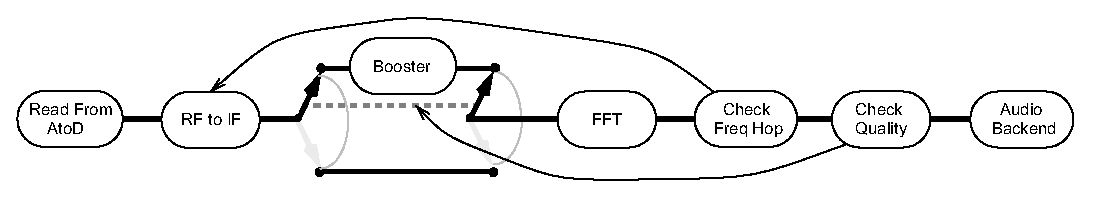
\includegraphics[width=\columnwidth]{Radio.eps}
\end{figure}

\clearpage
\begin{figure}
  \caption{An FIR filter in StreamIt.}
  \label{fig:firstreamit}
\end{figure}
\clearpage
\begin{figure}
  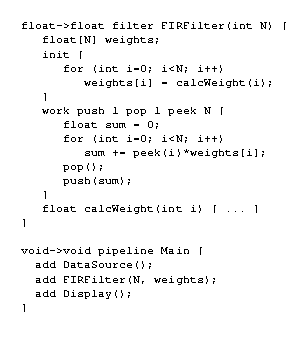
\includegraphics{fir-streamit.eps}
\end{figure}

\clearpage
\begin{figure}
  \caption{Stream structures supported by StreamIt: \texttt{pipeline} (left),
  \texttt{splitjoin} (middle), and a \texttt{feedbackloop} (right).}
  \label{fig:structuresp}
\end{figure}
\clearpage
\begin{figure}
  \begin{minipage}{0.46in}
  \centering
  \psfig{figure=pipeline.eps,width=0.46in} \\
  \end{minipage} 
  ~
  \begin{minipage}{1.3in}
  \centering
  \psfig{figure=splitjoin.eps,width=1.3in} \\
  \end{minipage}
  ~
  \begin{minipage}{1.02in}
  \centering
  \psfig{figure=feedback.eps,width=1.02in} \\
  \end{minipage} 
\end{figure}

\clearpage
\begin{figure}
  \caption{An optimized FIR filter in a procedural language.  A
  complicated loop nest is required to avoid mod functions and to use
  memory efficiently, and the structure of the loops depends on the
  data rates (e.g., BLOCK\_SIZE) within the stream.  An actual
  implementation might inline the calls to \texttt{step}.}
  \label{fig:firprocedural}
\end{figure}
\clearpage
\begin{figure}
  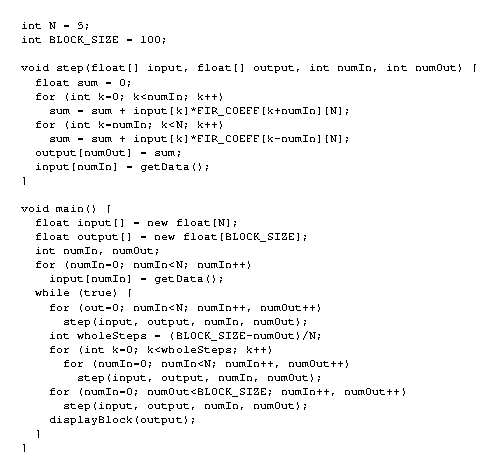
\includegraphics{fir-proc.eps}
\end{figure}

\clearpage
\begin{figure}
  \caption{An FIR filter in an object oriented language.  A ``pull
  model'' is used by each filter object to retrieve a chunk of data
  from its source, and straight-line code connects one filter to
  another.}
  \label{fig:firobject}
\end{figure}
\clearpage
\begin{figure}
  \includegraphics{fir-object.eps}
\end{figure}

\clearpage
\begin{figure}
  \caption{An echo effect in StreamIt.  Extra items are pushed on to
  \texttt{Delay}'s output tape in the \texttt{prework} function to
  cause the delay.}
  \label{fig:echo}
\end{figure}
\clearpage
\begin{figure}
  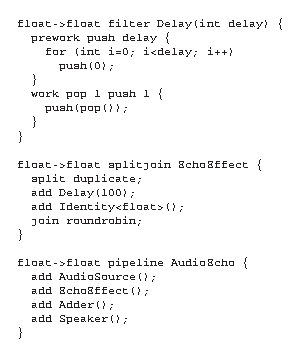
\includegraphics{echo.eps}
\end{figure}

\clearpage
\begin{figure}
  \caption{A \texttt{feedbackloop} version of Fibonnacci.}
\label{fig:feed}
\end{figure}
\clearpage
\begin{figure}
  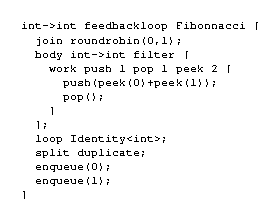
\includegraphics{fib-streamit.eps}
\end{figure}


\end{document}
